\documentclass{beamer}
\usetheme{metropolis}
\usepackage{graphicx}
\usepackage{boolexpr}
\usepackage{kpfonts}
\usepackage{caption}
\usepackage{wrapfig}
\usepackage{tkz-graph}
\usepackage{tikz}
\usepackage{chngcntr}
\usepackage[labelformat=empty]{caption}
\usepackage[official]{eurosym}

\usepackage[math]{iwona}
\usepackage{scalerel}
\def\lVert{\mid\!\mid}
\def\rVert{\mid\!\mid}

\usepackage[normalem]{ulem}
\newcommand{\Adj}{\mathbf{A}}

\usepackage{custom}
\usepackage{amsfonts}
\newcommand{\jsrcodepath}{../../latex/images}
\usepackage{jsr}

\usepackage{framed}

\newcommand\Wider[2][3em]{%
\makebox[\linewidth][c]{%
  \begin{minipage}{\dimexpr\textwidth+#1\relax}
  \raggedright#2
  \end{minipage}%
  }%
}

\newcommand{\aeur}{\alpha_\text{\euro}}
\newcommand{\adol}{\alpha_\$}
\newcommand{\apou}{\alpha_\text{\pounds}}

\newcommand{\cssystemtikz}[2]{
  \begin{center}
    \begin{tikzpicture}[x=#1,y=#2]
      \Vertex{1}
      \NO[unit=4](1){2}
      \SOEA[unit=2](2){3}
      \EA[unit=2](3){4}
      \tikzset{EdgeStyle/.style = {->}}
      \tikzset{LoopStyle/.style = {->}}
      \tikzset{EdgeStyle/.append style = {bend right=18}}
      \Edge[label=1](1)(3)
      \Edge[label=3](1)(2)
      \Edge[label=2](2)(1)
      \Edge[label=1](2)(3)
      \Edge[label=2](3)(1)
      \Edge[label=3](3)(2)
      \Edge[label=4](3)(4)
      \draw[thick,->] (3) to [out=115,in=65,looseness=20] node [midway, fill=white] {1} (3);
      \Edge[label=1](4)(3)
    \end{tikzpicture}
  \end{center}
}

\title{Generating unstable trajectories for Switched Systems via Dual Sum-Of-Squares techniques}
\date{}
\author{Beno\^it Legat}
\institute{Institute of Information and Communication Technologies, Electronics and Applied Mathematics (ICTEAM),\\
           Universit\'e catholique de Louvain (UCL)\\\\
           Based on joint work with Rapha\"el M. Jungers (UCL)
           and Pablo A. Parrilo (MIT)}

\begin{document}
  \maketitle
  \begin{frame}
    \tableofcontents
  \end{frame}
  \section{Introduction}
  \begin{frame}
      \frametitle{Motivation (from a Simulation viewpoint)}
      Analysis of integration method for $\dot{x} = Ax$ equivalent to analysis of dynamical systems\footnote{Based on joint work with Cl\'audio Gomes from the University of Antwerp}:
      \begin{center}
          \fbox{\parbox[m][9em][t]{0.33\textwidth}{
              Euler method:
              \begin{align*}
                  x_{k+1} &= x_k + h A x_k
              \end{align*}
              Midpoint method:
              \begin{align*}
                  x_{k+1} &= x_k + h A (x_k + \frac{h}{2}Ax_k)
              \end{align*}
          }}%
          $\Longleftrightarrow$%
          \fbox{\parbox[m][9em][t]{0.33\textwidth}{
              Euler method:
              \begin{align*}
                  e_{k+1} &= (I + hA)e_k + e_{\mathrm{local}}
              \end{align*}
              Midpoint method:
              \begin{align*}
                  e_{k+1} &= \Big(I + hA + \frac{h}{2}A^2\Big)e_k + e_{\mathrm{local}}
              \end{align*}
          }}
      \end{center}
      \uncover<2->{What happens if we \alert{switch} between the methods or step sizes ?}
      \uncover<3>{How can we compute the set of allowed switching sequences ?}
      \vspace{1em}
  \end{frame}

  \begin{frame}
      \frametitle{Example}
      Consider
      \begin{align*}
          A & =
          \begin{bmatrix}
              0 & 2\\
              0 & 0
          \end{bmatrix}&
          B & =
          \begin{bmatrix}
              0 & 0\\
              2 & 0
          \end{bmatrix}
      \end{align*}
      We have
      \begin{align*}
          \lim_{k \to \infty}& A \cdot A \cdot A \cdots = 0,&
          \lim_{k \to \infty}& B \cdot B \cdot B \cdots = 0,
      \end{align*}
      (in fact, $A$ and $B$ are nilpotent, so $A^2 = B^2 = 0$), but...
      \uncover<2->{
          \[ \lim_{k \to \infty} \norm{A \cdot B \cdot A \cdot B \cdots} = \infty \qquad \qquad (!) \]
      }
      \uncover<3>{
          The asymptotic growth rate of this sequence is 2, i.e.
          \[ \lim_{k \to \infty} \norm{(A \cdot B)^{\frac{k}{2}}}^{\frac{1}{k}} = 2 \]
      }
  \end{frame}

  \begin{frame}
      \frametitle{Joint spectral radius}
      Given a set of $n \times n$ matrices $\Sigma = \{A_1,\ldots,A_m\}$,
      what is the maximum ``growth rate'' that can be achieved by \alert{arbitrary switching}?
      \[ \rho(\Sigma) := \limsup_{k\to\infty} \max_{\sigma \in \{1,\ldots,m\}} \norm{A_{\sigma_k} \cdots A_{\sigma_2}A_{\sigma_1}}^{1/k}. \]

      Appeared in several different contexts: linear algebra (Rota-Strang 1960), wavelets (Daubechies-Lagarias 1992),
      switched linear systems, etc.

      \begin{itemize}
          \item If $m = 1$, ``standard'' spectral radius $\rho(A_1) = \max_i |\lambda_i|$.
          \item If $m \geq 2$, much more complicated...
      \end{itemize}
  \end{frame}

  \begin{frame}{Joint spectral radius is hard}
      Determining if $\rho(\Sigma) \leq 1$ is \alert{NP-hard} (Tsitsiklis \& Blondel 1997).

      \uncover<2->{Determining if $\rho(\Sigma) \leq 1$ is \alert{undecidable} (Blondel \& Tsitsiklis 2000).}

      \uncover<3->{Related work by Gurvitz (1995), Kozyakin, Barabanov, Wang-Lagarias ``finiteness conjecture'', Blondel-Nesterov, Theys, Jungers, etc...}

      \uncover<4->{
          Still, how to compute/approximate $\rho(\Sigma)$?

          What approximation guarantees can we have?

          How to produce ``bad'' switching sequences?
      }
  \end{frame}

  \begin{frame}{\only<2->{Constrained }Switched Systems}
    \begin{minipage}{0.23\textwidth}
      \[ x_{k+1} = A_{\sigma_k} x_k \]
      where \[A_{\sigma_k} \in \mathcal{M} \subseteq \R^{n \times n}.\]
    \end{minipage}
    \uncover<2->{%
      \begin{minipage}{0.75\textwidth}
        \cssystemtikz{50}{30}
      \end{minipage}
    }
    \begin{block}{\only<2->{Constrained }Joint Spectral Radius}
        \[ \only<1>{\jsr}\only<2>{\cjsr} = \lim_{k \to \infty} \max \norm{A_{\sigma_k} \cdots A_{\sigma_1}}^{1/k}.
      \]
      \uncover<2->{$\sigma_1, \ldots, \sigma_k$ is a path.}
    \end{block}
  \end{frame}

  \begin{frame}{Adjacency matrix}
    \Wider{\cssystemtikz{40}{20}%
      \uncover<2->{\[ \rho(\Adj) = \lim_{k \to \infty} \norm{\Adj^k}^{1/k}. \]}%
    \begin{minipage}{0.35\textwidth}
      \begin{align*}
        \only<1-3>{
          \Adj & =
          \begin{pmatrix}
            0 & 1 & 1 & 0\\
            1 & 0 & 1 & 0\\
            1 & 1 & 1 & 1\\
            0 & 0 & 1 & 0
          \end{pmatrix}.
        }
        \only<4>{
          \Adj^2 & =
          \begin{pmatrix}
            2 & 1 & 2 & 1\\
            1 & 2 & 2 & 1\\
            2 & 2 & 4 & 1\\
            1 & 1 & 1 & 1
          \end{pmatrix}.
        }
        \only<5>{
          \Adj^3 & =
          \begin{pmatrix}
            3 & 4 & 6 & 2\\
            4 & 3 & 6 & 2\\
            6 & 6 & 9 & 4\\
            2 & 2 & 4 & 1
          \end{pmatrix}.
        }
      \end{align*}
    \end{minipage}
    \begin{minipage}{0.6\textwidth}
      \begin{align*}
        \only<3>{
          \norm{\Adj}_\infty & = \max
          \begin{pmatrix}
            0 + 1 + 1 + 0\\
            1 + 0 + 1 + 0\\
            1 + 1 + 1 + 1\\
            0 + 0 + 1 + 0
          \end{pmatrix} =
          \begin{pmatrix}
            2\\2\\4\\1
          \end{pmatrix}.%
        }
        \only<4>{
          \norm{\Adj^2}_\infty & = \max
          \begin{pmatrix}
            2 + 1 + 2 + 1\\
            1 + 2 + 2 + 1\\
            2 + 2 + 4 + 1\\
            1 + 1 + 1 + 1
          \end{pmatrix} =
          \begin{pmatrix}
            6\\6\\9\\4
          \end{pmatrix}.%
        }
        \only<5>{
          \norm{\Adj^3}_\infty & = \max
          \begin{pmatrix}
            3 + 4 + 6 + 2\\
            4 + 3 + 6 + 2\\
            6 + 6 + 9 + 4\\
            2 + 2 + 4 + 1
          \end{pmatrix} =
          \begin{pmatrix}
            15\\15\\25\\9
          \end{pmatrix}.
        }
      \end{align*}
  \end{minipage}}
  \end{frame}


  \section{Lyapunov functions and their Sum of Squares Approximation}

  \begin{frame}
      \frametitle{Lyapunov function}
      \begin{block}{Theorem}
          Let $f(x)$ be a strictly positive homogeneous function,
          that satisfies
          \[ f(A_\sigma x) \leq \gamub f(x), \qquad \forall x \in \R^n, \sigma = 1, \ldots, m. \]
          Then $\jsr \leq \gamub$.
      \end{block}
  \end{frame}

  \begin{frame}
      \frametitle{Using SOS}
      We need a homogeneous polynomials $p(x)$ that satisfies
      \[ p(x) \geq 0, \qquad \gamub^{2d}p(x) - p(A_\sigma x) \geq 0 \quad \sigma = 1, \ldots, m. \]
      While this is not tractable, we can use instead
      \[ p(x) \text{ is SOS}, \qquad \gamub^{2d}p(x) - p(A_\sigma x) \text{ is SOS}\quad \sigma = 1, \ldots, m. \]
      Then $\jsr \leq \ujsrsos := \gamub$.

      For fixed $\gamub$, this is an SOS program, can be solved using an SDP solver.
  \end{frame}

  \begin{frame}{Example}
      Based on (Ando and Shih 98). Consider the two matrices:
      \[
          A_1 =
          \begin{bmatrix}
              1 & 0\\
              1 & 0
          \end{bmatrix},
          A_2 =
          \begin{bmatrix}
              0 & 1\\
              0 & -1
          \end{bmatrix},
      \]
      \begin{itemize}
          \item The true spectral radius is $\rho(A_1, A_2) = 1$.
          \item A common quadratic Lyapunov function (i.e. $d = 2$),
              gives $\rho(A_1, A_2) \leq \sqrt{2}$.
      \end{itemize}
  \end{frame}

  \begin{frame}{Example (cont.)}
      \begin{columns}
          \begin{column}{.6\textwidth}
              A quartic SOS Lyapunov function is enough to prove an upper bound
              of $1+\epsilon$ for \emph{every} $\epsilon > 0$, since
              \[ V(x) = (x_1^2 - x_2^2)^2 + \epsilon (x_1^2 + x_2^2)^2 \]
          \end{column}
          \begin{column}{.4\textwidth}
              \includegraphics[trim=0cm 0cm 0cm .6cm, clip, width=\textwidth]{polynomial.png}
          \end{column}
      \end{columns}
      satisfies
      \begin{align*}
          (1+\epsilon)V(x) - V(A_1x) &= (x_2^2-x_1^2 + \epsilon(x_1^2+x_2^2))^2\\
          (1+\epsilon)V(x) - V(A_2x) &= (x_1^2-x_2^2 + \epsilon(x_1^2+x_2^2))^2.
      \end{align*}

      \uncover<2>{What (if anything) can we say about approximation properties?}
  \end{frame}

  \begin{frame}
      \frametitle{SOS Guarantees}
      The degree-$d$ SOS upper bound for $\rho(A_1, \ldots,A_m)$ satisfies
      \[ \eta^{-\frac{1}{2d}} \ujsrsos \leq \jsr \leq \ujsrsos \]
      where $\eta = \min\Big\{m, {n+d-1 \choose d}\Big\}$.
      \begin{itemize}
          \item As degree $d \to \infty$, approx. ratio goes to 1!
          \item For unbounded $m$, related to Barvinok/John's ellispoid.
          \item For fixed $n$, proof based on Lyapunov iteration.
      \end{itemize}
      \uncover<2>{
          But...
          \begin{itemize}
              \item How to generalize to \emph{constrained} switching?
              \item How to produce ``bad'' switching sequences?
          \end{itemize}
      }
      \vfill
      {\scriptsize
      P.A. Parrilo and A. Jadbabaie,
      Approximation of the joint spectral radius using sum of squares,
      \emph{Linear Algebra and its Applications},
      Vol. 428, No. 10, pp.~2385--2402, 2008.
      }
  \end{frame}

  \begin{frame}{Constrained Switching Systems and multi-Lyapunov}
      \null{}
      \vspace{-2.5em}
      \begin{center}
        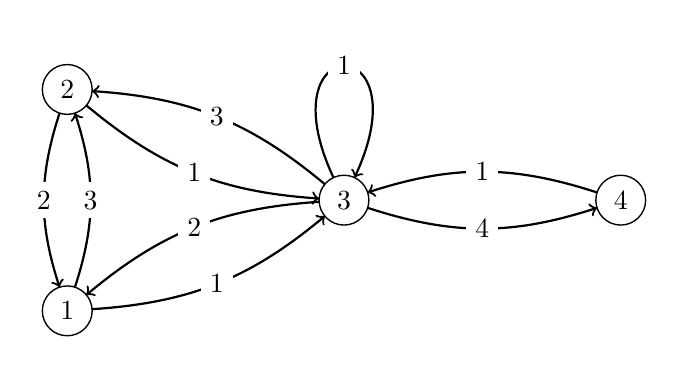
\begin{tikzpicture}[x=50,y=20]
          \Vertex{1}
          \NO[unit=4](1){2}
          \SOEA[unit=2](2){3}
          \EA[unit=2](3){4}
          \tikzset{EdgeStyle/.style = {->}}
          \tikzset{LoopStyle/.style = {->}}
          \tikzset{EdgeStyle/.append style = {bend right=18}}
          \only<1-2>{
            \Edge[label=1](1)(3)
            \Edge[label=3](1)(2)
            \Edge[label=2](2)(1)
            \Edge[label=1](2)(3)
            \Edge[label=2](3)(1)
            \Edge[label=3](3)(2)
            \Edge[label=4](3)(4)
            \draw[thick,->] (3) to [out=115,in=65,looseness=20] node [midway, fill=white] {1} (3);
            \Edge[label=1](4)(3)
          }
        \end{tikzpicture}
      \end{center}
      \uncover<2->{
          \[ u \to_\sigma v \qquad f_v(A_{\sigma}x) \leq \gamub f_u(x). \]
          The degree-$d$ SOS upper bound satisfies
          \[ \eta^{-\frac{1}{2d}} \jsrsos \leq \cjsr \leq \jsrsos \]
          where $\eta = {n+d-1 \choose d}$.
      }

      \vfill

      {\scriptsize
      M. Philippe, R. Essick, G. Dullerud and R.M. Jungers, Stability of discrete-time switching systems with constrained switching sequences, \emph{arXiv preprint arXiv:1503.06984}, 2015}
  \end{frame}
  \begin{frame}{multi-Lyapunov functions}
    \Wider{
      \begin{center}
        \tabulinesep=0.5mm
        \begin{tabu}{{X[.7,c,m]X[c,m]X[c,m]X[c,m]X[c,m]}}
          & Node 1 & Node 2 & Node 3 & Node 4\\
          \PrimalFig{2}{1}
          \PrimalFig{4}{2}
          \PrimalFig{12}{6}
        \end{tabu}
      \end{center}
    }
  \end{frame}
  \begin{frame}{SOS Program}
    \begin{align*}
      \inf \gamub\\
      p_v(x) & \text{ is SOS} & \forall v \in \Nodes\\
      \gamub^{2d} p_u(x) - p_v(A_\sigma x) & \text{ is SOS} & \forall (u, v, \sigma) \in \Arcs.
    \end{align*}

      \uncover<2>{
          Last but not least...
          \begin{itemize}
              \item How to produce ``bad'' switching sequences?
          \end{itemize}
      }
  \end{frame}

  \section{Measures containing unstable trajectories and their moment relaxation}

  \begin{frame}{Measures containing unstable trajectories}
      \begin{block}{Theorem}
          Let $\mu_{\sigma}$, $\sigma=1, \ldots, m$, be measures on $\mathbb{S}^{n-1}$,
          that satisfies
          \[ \sum_{\sigma = 1}^m \Exp_{\mu_\sigma}[f(A_\sigma x)] \geq \gamlb \sum_{\sigma = 1}^m \Exp_{\mu_\sigma}[f(x)], \quad \forall \text{ nonnegative homogeneous } f \]
          and at least one of the expectations is nonzero.

          Then  $\jsr \geq \gamlb$.
      \end{block}
  \end{frame}

  \begin{frame}
    \frametitle{Example: Arbitration in Economy}
    \begin{center}
      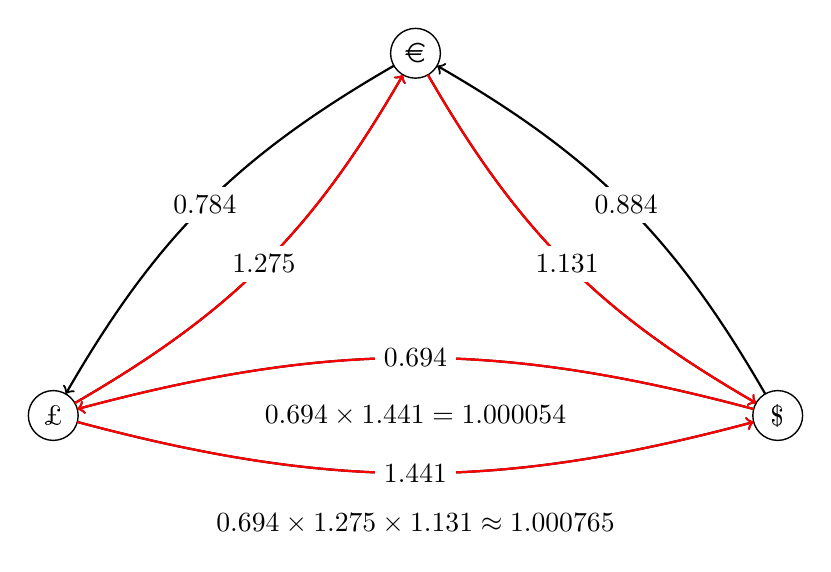
\begin{tikzpicture}[scale=2.3]
        \Vertex[L=\euro]{1}
        \SOEA[L=\$,unit=2](1){2}
        \SOWE[L=\pounds,unit=2](1){3}
        \tikzset{EdgeStyle/.style = {->}}
        \tikzset{LoopStyle/.style = {->}}
        \tikzset{EdgeStyle/.append style = {bend right=15}}
        \Edge[label=0.884](2)(1)
        \Edge[label=0.784](1)(3)
        \uncover<1,2>{
          \Edge[label=1.131](1)(2)
          \Edge[label=1.275](3)(1)
        }
        \uncover<1>{
          \Edge[label=0.694](2)(3)
        }
        \uncover<1,3>{
          \Edge[label=1.441](3)(2)
        }
        \uncover<2>{
          \Edge[label=1.441,color=red](3)(2)
          \node at (0,-2) {$0.694 \times 1.441 = 1.000054$};
        }
        \uncover<2->{
          \Edge[label=0.694,color=red](2)(3)
        }
        \uncover<3>{
          \Edge[label=1.131,color=red](1)(2)
          \Edge[label=1.275,color=red](3)(1)
          \node at (0,-2.6) {$0.694 \times 1.275 \times 1.131 \approx 1.000765$};
        }
      \end{tikzpicture}
    \end{center}
  \end{frame}
  \begin{frame}
    \frametitle{Let's make it stable}
    \begin{center}
      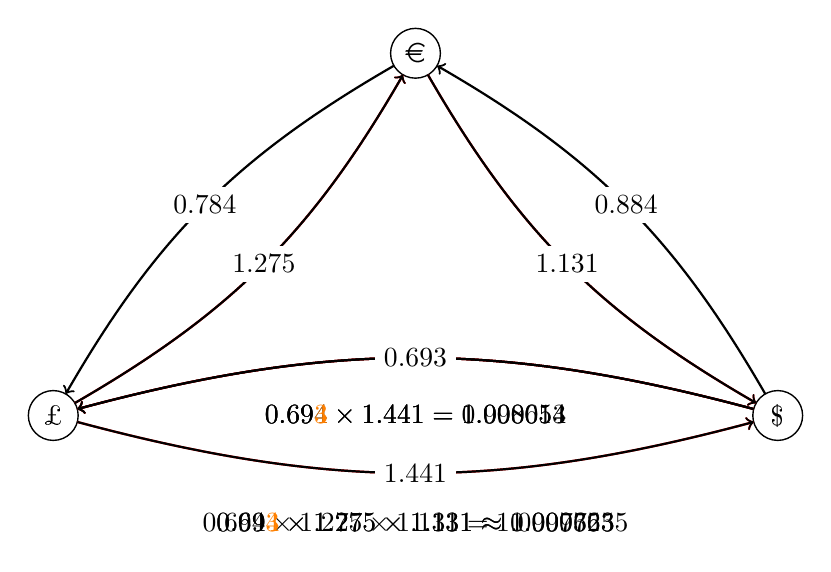
\begin{tikzpicture}[scale=2.3]
        \Vertex[L=\euro]{1}
        \SOEA[L=\$,unit=2](1){2}
        \SOWE[L=\pounds,unit=2](1){3}
        \tikzset{EdgeStyle/.style = {->}}
        \tikzset{LoopStyle/.style = {->}}
        \tikzset{EdgeStyle/.append style = {bend right=15}}
        \Edge[label=0.884](2)(1)
        \Edge[label=0.784](1)(3)
        \uncover<1,2>{
          \Edge[label=1.441,color=red](3)(2)
          \Edge[label=1.131,color=red](1)(2)
          \Edge[label=1.275,color=red](3)(1)
        }
        \uncover<1>{
          \Edge[label=0.694,color=red](2)(3)
          \node at (0,-2) {$0.694 \times 1.441 = 1.000054$};
          \node at (0,-2.6) {$0.694 \times 1.275 \times 1.131 = 1.00076535$};
        }
        \uncover<2>{
          \Edge[label=0.69\protect\color{orange}4,color=red](2)(3)
          \node at (0,-2) {$0.69\textcolor{orange}{4} \times 1.441 = 1.000054$};
          \node at (0,-2.6) {$0.69\textcolor{orange}{4} \times 1.275 \times 1.131 \approx 1.000765$};
        }
        \uncover<3>{
          \Edge[label={0.69\protect\color{orange}3}](2)(3)
          \node at (0,-2) {$0.69\textcolor{orange}{3} \times 1.441 = 0.998613$};
          \node at (0,-2.6) {$0.69\textcolor{orange}{3} \times 1.275 \times 1.131 \approx 0.999323$};
        }
        \uncover<3->{
          \Edge[label=1.131](1)(2)
          \Edge[label=1.275](3)(1)
          \Edge[label=1.441](3)(2)
        }
        \uncover<4>{
          \Edge[label={0.693}](2)(3)
        }
      \end{tikzpicture}
    \end{center}
  \end{frame}

  \begin{frame}{Lyapunov functions in the scalar case}
    \Wider{
      \begin{center}
        \begin{tikzpicture}[scale=2.3]
          \only<1>{
            \Vertex[L=$\aeur$]{1}
            \SOEA[L=$\adol$,unit=2](1){2}
            \SOWE[L=$\apou$,unit=2](1){3}
          }
          \only<2>{
            \tikzset{VertexStyle/.append style = {minimum size = 2.262cm}}
            \Vertex[L={$\aeur=1.131$}]{1}
            \tikzset{VertexStyle/.append style = {minimum size = 2cm}}
            \SOEA[L={$\adol=1$},unit=2](1){2}
            \tikzset{VertexStyle/.append style = {minimum size = 2.88405cm}}
            \SOWE[L={$\apou=1.442025$},unit=2](1){3}
          }
          \tikzset{EdgeStyle/.style = {->}}
          \tikzset{LoopStyle/.style = {->}}
          \tikzset{EdgeStyle/.append style = {bend right=15}}
          \Edge[label=$\aeur \leq 0.884 \cdot \adol$](2)(1)
          \Edge[label=$\apou \leq 0.784 \cdot \aeur$](1)(3)
          \Edge[label=$\adol \leq 1.131 \cdot \aeur$](1)(2)
          \Edge[label=$\aeur \leq 1.275 \cdot \apou$](3)(1)
          \Edge[label=$\adol \leq 1.441 \cdot \apou$](3)(2)
          \Edge[label=$\apou \leq 0.693 \cdot \adol$](2)(3)
        \end{tikzpicture}
      \end{center}
    }
  \end{frame}
  \begin{frame}{Measures containing arbitrages (LP dual of Lyapunov program)}
    \Wider[4em]{
    \begin{center}
      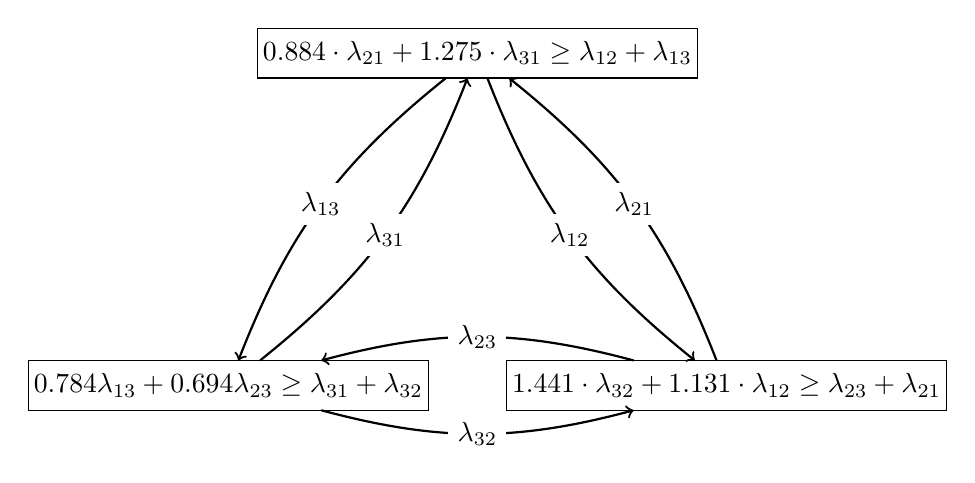
\begin{tikzpicture}[x=45, y=60]
        \tikzset{VertexStyle/.append style = {shape=rectangle}}
        \Vertex[L=$0.884 \cdot \lambda_{21} + 1.275 \cdot \lambda_{31} \geq \lambda_{12} + \lambda_{13}$]{1}
        \SOEA[L={$1.441 \cdot \lambda_{32} + 1.131 \cdot \lambda_{12} \geq \lambda_{23} +\lambda_{21}$},unit=2](1){2}
          \SOWE[L={$0.784 \lambda_{13} + 0.694 \lambda_{23} \geq \lambda_{31} + \lambda_{32}$},unit=2](1){3}
        \tikzset{EdgeStyle/.style = {->}}
        \tikzset{LoopStyle/.style = {->}}
        \tikzset{EdgeStyle/.append style = {bend right=15}}
        \Edge[label=$\lambda_{21}$](2)(1)
        \Edge[label=$\lambda_{13}$](1)(3)
        \Edge[label=$\lambda_{12}$](1)(2)
        \Edge[label=$\lambda_{31}$](3)(1)
        \Edge[label=$\lambda_{32}$](3)(2)
        \Edge[label=$\lambda_{23}$](2)(3)
      \end{tikzpicture}
  \end{center}
  }
      Solutions are:
      \uncover<2->{Any conic combinations of
      \[ (\lambda_{23}, \lambda_{32}) = (1, 0.694) \text{ and } (\lambda_{23}, \lambda_{31}, \lambda_{12}) = (1, 0.694, 0.694\times1.274) \]
      }
      \uncover<3>{The measures can contain \alert{several} different trajectories!}
  \end{frame}

  \begin{frame}{Extracting trajectories from measures}
      We say that the measures contain only one trajectory if for every $\hat{x}$, at \emph{most} one of the terms of the LHS of
      \[ \sum_{\sigma = 1}^m \Exp_{\mu_\sigma}[f(A_\sigma x)] \geq \gamlb \sum_{\sigma = 1}^m \Exp_{\mu_\sigma}[f(x)], \]
      is nonzero with $f(x) = \delta_{\hat{x}}(x)$.

      If the measures contain only one trajectory, we can extract it as follows
      \begin{itemize}
          \item Take $\sigma_0$, $x_0$ such that $\Exp_{\mu_{\sigma_0}}[\delta_{x_0}] > 0$.
          \item Set $\sigma_{k+1}$ to the \alert{only} $\sigma$ such that $\Exp_{\mu_{\sigma}}[\delta_{x_k}(A_\sigma x)] > 0$.
          \item Set $x_{k+1} = A_{\sigma_{k+1}}^{-1}x_k$.
      \end{itemize}
      Remark: the trajectory is built in \alert{backward} order.
  \end{frame}

  \begin{frame}{Moment Program}
      Given the moments of a measure $\mu$ up to degree $2d$,
      we can write the constraint
      \[
          \Exp_{\mu}[p(x)] = \int_{\mathbb{S}^{n-1}} p(x) \dif \mu \geq 0, \qquad \forall p(x) \text{ SOS of degree }2d.
      \]
      as Semidefinite Programming constraints [Lasserre 2001].

      The moment relaxation of our program is:
      \begin{align}
          \notag
          \sup_{\mu_{uv\sigma} \in \Soshd, \gamlb \in \R} \gamlb\\
          \notag
          \sum_{(u,v,\sigma) \in \Arcs} \Exp_{\mu_{uv\sigma}}[p(A_\sigma x)] & \succeq \gamlb^{2d} \sum_{(v,w,\sigma) \in \Arcs} \Exp_{\mu_{vw\sigma}}[p(x)], \forall p(x) \in \Sosh, \forall v \in \Nodes,\\
          \notag
          \sum_{(u,v,\sigma) \in \Arcs} \Exp_{\mu_{uv\sigma}}\Big[\sum_{i=1}^n x_i^{2d}\Big] & = 1.
      \end{align}
  \end{frame}

  \begin{frame}{Why is it a relaxation ?}
      \Wider{
          The Semidefinite Programming constraints on the trunctated moments of $\mu_\sigma$ are necessary for the existence of a measure with those moments,
      and \alert{any} value of the moments of higher degree (not necessarily 0).

      In the Common Quadratic Lyapunov Function case, i.e. $2d = 2$, those conditions are necessary and sufficient.
      \begin{itemize}
          \item For every truncated moments, we can find a $\mu_\sigma$ that has these moments.
          \item And there exists a slack variable $\mu_{\mathrm{slack}}$ such that
              \[ \sum_{\sigma=1}^m \Exp_{\mu_\sigma}[p(A_\sigma x)] - \gamlb^{2d} \sum_{\sigma = 1}^m \Exp_{\mu_\sigma}[p(x)] = \Exp_{\mu_{\mathrm{slack}}}, \forall p(x) \in \Sosh, \]
              so
              \[ \sum_{\sigma=1}^m \mathcal{A}_\sigma \mu_\sigma - \gamlb^{2d} \sum_{\sigma = 1}^m \mu_\sigma \only<1>{=}\only<2>{\text{ has the same trunctated moments than }} \mu_{\mathrm{slack}} \]
      \end{itemize}
      }
  \end{frame}

  \begin{frame}{When we have luck}
      If we find measures such that
      \[ \sum_{\sigma=1}^m \mathcal{A}_\sigma \mu_\sigma - \gamlb^{2d} \sum_{\sigma = 1}^m \mu_\sigma \]
      is a measure then $\gamlb \leq \jsr$.

      \begin{itemize}
          \item In fact, the moment and lyapunov programs are dual, so $\gamlb = \gamub$.
              Therefore, we have $\gamlb = \jsr = \gamub$.
          \item In practice we can try to decompose the $\mu_\sigma$'s as a sum of diracs. But it can only works if the system has the finiteness property.
      \end{itemize}
  \end{frame}

  \begin{frame}{Example}
      Let
      \[ \A = \{ A_1 = e_1e_2^\Tr , A_2 = e_2e_1^\Tr  \} \]

      A Lyapunov with $2d = 2$ and $\gamub = 1$ is given by $\norm{x}_2$.

      Measures with $2d = 2$ and $\gamlb = 1$ are given by $\mu_1 = \delta_{(0,1)}$ and $\mu_2 = \delta_{(1,0)}$.

      \begin{center}
      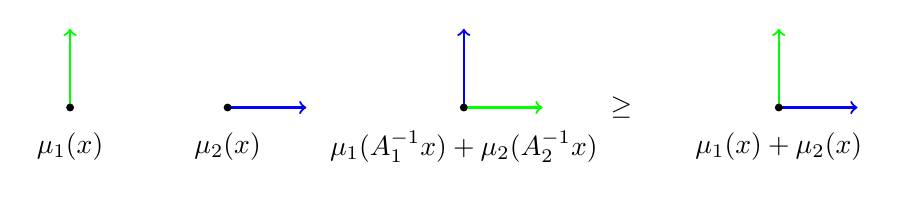
\begin{tikzpicture}
          \begin{scope}[shift={(-7,0)}]
              \draw[thick,->,green] (0,0) to (0,1);
              \fill (0,0) circle(.05);
              \node at (0,-.5) {$\mu_1(x)$};
          \end{scope}

          \begin{scope}[shift={(-5,0)}]
              \draw[thick,->,blue] (0,0) to (1,0);
              \fill (0,0) circle(.05);
              \node at (0,-.5) {$\mu_2(x)$};
          \end{scope}

          \begin{scope}[shift={(-2,0)}]
              \draw[thick,->,green] (0,0) to (1,0);
              \draw[thick,->,blue] (0,0) to (0,1);
              \fill (0,0) circle(.05);
              \node at (0,-.5) {$\mu_1(A_1^{-1}x) + \mu_2(A_2^{-1}x)$};
          \end{scope}

          \begin{scope}[shift={(0,0)}]
              \node at (0,0) {$\geq$};
          \end{scope}

          \begin{scope}[shift={(2,0)}]
              \draw[thick,->,green] (0,0) to (0,1);
              \draw[thick,->,blue] (0,0) to (1,0);
              \fill (0,0) circle(.05);
              \node at (0,-.5) {$\mu_1(x) + \mu_2(x)$};
          \end{scope}
      \end{tikzpicture}
  \end{center}
  \end{frame}

  \begin{frame}{Building a high growth sequence}
      \vspace{-1em}
    \Wider{\[ \sum_{(u,v,\sigma) \in E} \Exp_{\mu_{uv\sigma}}[p(A_\sigma x)] \geq \gamlb^{2d}\sum_{(v,w,\sigma) \in \Arcs} \Exp_{\mu_{vw\sigma}}[p(x)], \qquad \forall v \in \Nodes, p(x) \text{ SOS}, \]
    \begin{center}
      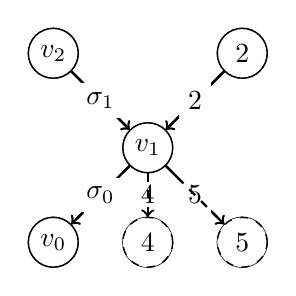
\begin{tikzpicture}
        \SetGraphUnit{1.2}
        \GraphInit[vstyle=Dijkstra]
        \SetUpEdge[style={->}]
        \uncover<1,2>{\Vertex[L=$v$]{0}}
        \uncover<3->{\Vertex[L=$v_1$]{0}}
        \uncover<1,2,3>{\NOWE[L=$1$](0){4};}
        \uncover<4>{\NOWE[L=$v_2$](0){4};}
        \uncover<1-3>{\NOEA[L=$2$](0){5};}
        \uncover<1,2>{
          \SOWE[L=$3$](0){10};
          \SO[L=$4$](0){11};
          \SOEA[L=$5$](0){12};
        }
        \uncover<3->{
          \SOWE[L=$v_0$](0){10};
          \tikzset{VertexStyle/.append style = {dashed}}
          \SO[L=$4$](0){11};
          \SOEA[L=$5$](0){12};
        }
        \uncover<4>{\NOEA[L=$2$](0){5};}
        \uncover<1-3>{\Edge[label=$1$](4)(0);}
        \uncover<4>{\Edge[label=$\sigma_1$](4)(0);}
        \uncover<1-3>{\Edge[label=$2$](5)(0);}
        \uncover<1,2>{
          \Edge[label=$3$](0)(10);
          \Edge[label=$4$](0)(11);
          \Edge[label=$5$](0)(12);
        }
        \uncover<3->{
          \tikzset{EdgeStyle/.append style = {dashed}}
          \Edge[label=$\sigma_0$](0)(10);
          \Edge(0)(11);
          \Edge(0)(12);
        }
        \uncover<4>{\Edge[label=$2$](5)(0);}
      \end{tikzpicture}
    \end{center}
      Construct sequence \emph{backwards}, using ``best expectation'':
    \begin{align*}
      \uncover<2->{\Exp_{\mu_{1v1}}[p(A_1 x)] + \Exp_{\mu_{2v2}}[p(A_2 x)] & \geq \gamlb^{2d}(\Exp_{\mu_{v33}}[p(x)] + \Exp_{\mu_{v44}}[p(x)] + \Exp_{\mu_{v55}}[p(x)]),\\}
      \uncover<3->{\Exp_{\mu_{1v_11}}[p(A_1 x)] + \Exp_{\mu_{2v_12}}[p(A_2 x)] & \geq \gamlb^{2d}\Exp_{\mu_{v_1v_0\sigma_0}}[p(x)],\\}
      \uncover<4>{\Exp_{\mu_{v_2v_1\sigma_1}}[p(A_1 x)] & \geq \frac{1}{2} \gamlb^{2d}\Exp_{\mu_{v_1v_0\sigma_0}}[p(x)].}
    \end{align*}
  }
  \end{frame}
  \begin{frame}{Choice of polynomial}
      Initial $p_0(x)$ arbitrary (as long as it is strictly SOS).

    \[ p_{k+1}(x) = p_{k}(A_{\sigma_k}x) = p_0(A_{\sigma_1} \cdots A_{\sigma_k} x) \]

    \begin{center}
      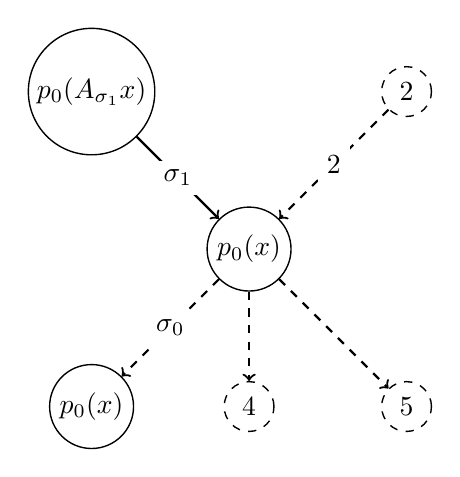
\begin{tikzpicture}
        \SetGraphUnit{2}
        \GraphInit[vstyle=Dijkstra]
        \SetUpEdge[style={->}]
        \Vertex[L=$p_0(x)$]{0}
        \NOWE[L=$p_0(A_{\sigma_1} x)$](0){4};
        \SOWE[L=$p_0(x)$](0){10};
        \tikzset{VertexStyle/.append style = {dashed}}
        \SO[L=$4$](0){11};
        \SOEA[L=$5$](0){12};
        \NOEA[L=$2$](0){5};
        \Edge[label=$\sigma_1$](4)(0);
        \tikzset{EdgeStyle/.append style = {dashed}}
        \Edge[label=$\sigma_0$](0)(10);
        \Edge(0)(11);
        \Edge(0)(12);
        \Edge[label=$2$](5)(0);
      \end{tikzpicture}
    \end{center}

  \end{frame}
  \begin{frame}{Algorithm and Guarantees}
    \begin{algorithmic}
      \STATE{Pick an arbitrary polynomial $p_0(x) \in \inte(\Sosh)$}
      \STATE{Pick an \arc{} $(v_1,v_0,\sigma_0) \in \Arcs$ such that $\Exp_{\mu_{v_1v_0\sigma_0}}[p_0(x)] > 0$}
      \STATE{Set $p_1(x) \leftarrow p_0(x)$}
      \FOR{$k = 1,2,\ldots$}
      \STATE $(v_{k+1},v_k,\sigma_k) \leftarrow \argmax_{(u,v_k,\sigma) \in \Arcs} \Exp_{\mu_{uv_k\sigma}}[p_k(A_\sigma x)]$
      \STATE $p_{k+1} \leftarrow p_k(A_{\sigma_k} x)$
      \ENDFOR
    \end{algorithmic}

    Let
    \[
        \theta_k \triangleq \Exp_{\mu_{v_{k+1}v_k\sigma_k}}[p_{0}(A_{\sigma_1} \cdots A_{\sigma_k}x)].
    \]
    We have
    \[ \theta_{k} \geq \frac{\gamlb^{2d}}{\din(v_k)} \theta_{k-1}. \]

    \uncover<2>{
      \hfill
      \[ \frac{\gamlb}{\norm{\Adj^\Tr}_\infty^{\frac{1}{2d}}} \leq \lim_{k \to \infty} \norm{A_{\sigma_1} \cdots A_{\sigma_k}}^{\frac{1}{k}}. \]
    }
  \end{frame}
  \begin{frame}{Let's try it}
    \begin{center}
      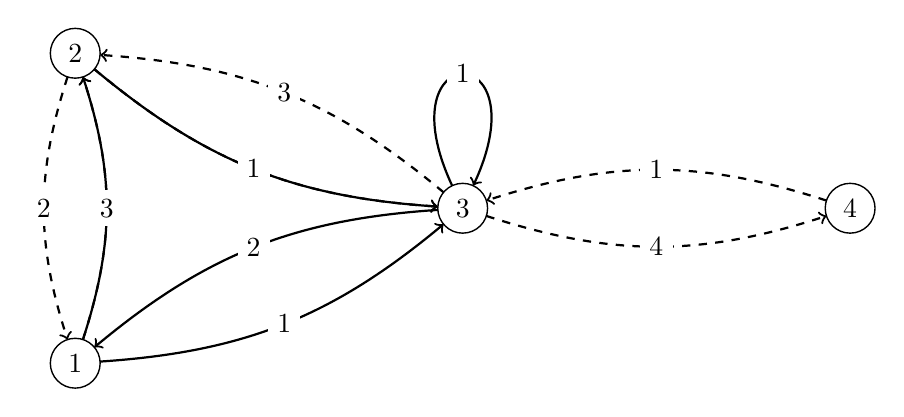
\begin{tikzpicture}[x=70,y=28]
        \Vertex{1}
        \NO[unit=4](1){2}
        \SOEA[unit=2](2){3}
        \EA[unit=2](3){4}
        \tikzset{EdgeStyle/.style = {->}}
        \tikzset{LoopStyle/.style = {->}}
        \tikzset{EdgeStyle/.append style = {bend right=18}}
        \Edge[label=1](1)(3)
        \Edge[label=2](3)(1)
        \draw[thick,->] (3) to [out=115,in=65,looseness=20] node [midway, fill=white] {1} (3);
        \uncover<2>{
          \Edge[label=3](1)(2)
          \Edge[label=1](2)(3)
        }
        \uncover<1>{
          \tikzset{EdgeStyle/.append style = {dashed}}
          \Edge[label=3](1)(2)
          \Edge[label=1](2)(3)
        }
        \tikzset{EdgeStyle/.append style = {dashed}}
        \Edge[label=2](2)(1)
        \Edge[label=3](3)(2)
        \Edge[label=4](3)(4)
        \Edge[label=1](4)(3)
      \end{tikzpicture}
      \hspace{1cm}
      \only<1>{
        $2d = 2$
        \[ 3 \to_2 1 \to_1 3 \to_2 1 \to_3 1 \to_1 3 \to_1 3 \to_1 3 \to_1 3 \to_1 3 \]
        $0.97\textcolor{red}{289}$
      }
      \only<2>{
        $2d = 12$
        \[ 3 \to_2 1 \to_1 3 \to_2 1 \to_3 2 \to_1 3 \to_1 3 \to_1 3 \to_1 3 \]
        $0.97\textcolor{green}{482}$
      }
    \end{center}
  \end{frame}
  \begin{frame}{Improvement}
    \only<1>{
      \begin{center}
      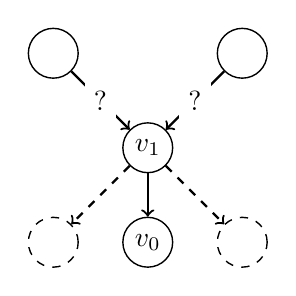
\begin{tikzpicture}
        \SetGraphUnit{1.2}
        \GraphInit[vstyle=Dijkstra]
        \SetVertexNoLabel
        \SetUpEdge[style={->}]
        \Vertex[NoLabel=false,L=$v_1$]{0}
        \NOWE(0){4};
        \NOEA(0){5};
        \SO[NoLabel=false,L=$v_0$](0){11};
        \tikzset{VertexStyle/.append style = {dashed}}
        \SOWE(0){10};
        \SOEA(0){12};
        \Edge[label=?](4)(0);
        \Edge[label=?](5)(0);
        \Edge(0)(11);
        \tikzset{EdgeStyle/.append style = {dashed}}
        \Edge(0)(10);
        \Edge(0)(12);
      \end{tikzpicture}
      \end{center}
    }
    \only<2>{
      \begin{center}
      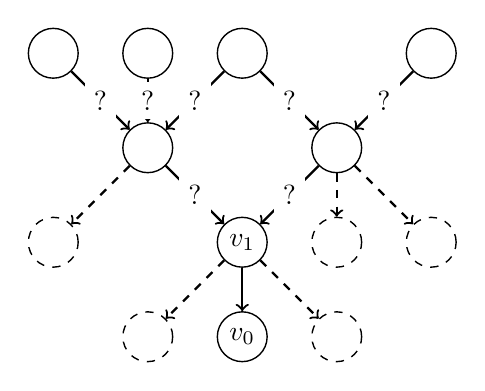
\begin{tikzpicture}
        \SetGraphUnit{1.2}
        \GraphInit[vstyle=Dijkstra]
        \SetVertexNoLabel
        \SetUpEdge[style={->}]
        \Vertex[NoLabel=false,L=$v_1$]{0}
        \NOWE(0){4};
        \NOEA(0){5};
        \NOWE(4){6};
        \NO  (4){7};
        \NOEA(4){8};
        \NOEA(5){9};
        \SO[NoLabel=false,L=$v_0$](0){11};
        \tikzset{VertexStyle/.append style = {dashed}}
        \SOWE(4){1};
        \EA(0){2};
        \EA(2){3};
        \SOWE(0){10};
        \SOEA(0){12};
        \Edge[label=?](6)(4);
        \Edge[label=?](7)(4);
        \Edge[label=?](8)(4);
        \Edge[label=?](8)(5);
        \Edge[label=?](9)(5);
        \Edge[label=?](4)(0);
        \Edge[label=?](5)(0);
        \Edge(0)(11);
        \tikzset{EdgeStyle/.append style = {dashed}}
        \Edge(4)(1);
        \Edge(5)(2);
        \Edge(5)(3);
        \Edge(0)(10);
        \Edge(0)(12);
      \end{tikzpicture}
      \end{center}
    }
  \end{frame}
  \begin{frame}{Improved guarantee}
      With horizon 1:
      \[ \frac{\gamlb}{\norm{\Adj^\Tr}_\infty^{\frac{1}{2d}}} \leq \lim_{k \to \infty} \norm{A_{\sigma_1} \cdots A_{\sigma_k}}^{\frac{1}{k}}. \]

    With horizon $l$:
    \[ \frac{\gamlb}{\norm{[\Adj^\Tr]^l}_\infty^{\frac{1}{2dl}}} \leq \lim_{k \to \infty} \norm{A_{\sigma_1} \cdots A_{\sigma_k}}^{\frac{1}{k}}. \]
  \end{frame}
  \begin{frame}{Let's try it}
    \begin{center}
      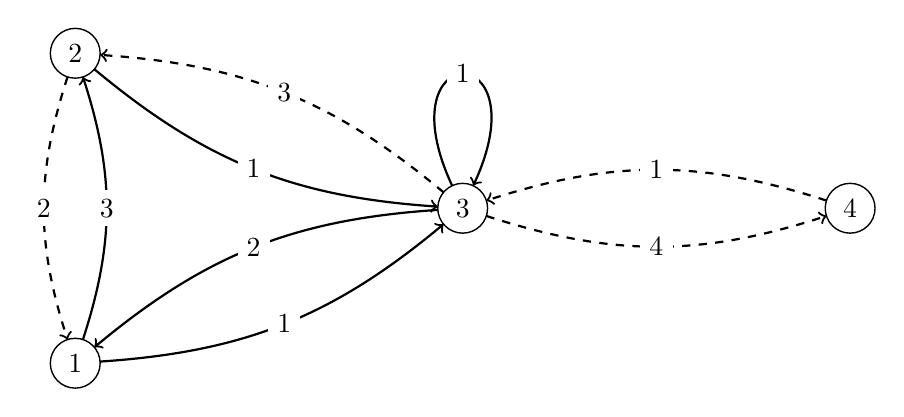
\begin{tikzpicture}[x=70,y=28]
        \Vertex{1}
        \NO[unit=4](1){2}
        \SOEA[unit=2](2){3}
        \EA[unit=2](3){4}
        \tikzset{EdgeStyle/.style = {->}}
        \tikzset{LoopStyle/.style = {->}}
        \tikzset{EdgeStyle/.append style = {bend right=18}}
        \Edge[label=1](1)(3)
        \Edge[label=2](3)(1)
        \draw[thick,->] (3) to [out=115,in=65,looseness=20] node [midway, fill=white] {1} (3);
        \Edge[label=3](1)(2)
        \Edge[label=1](2)(3)
        \tikzset{EdgeStyle/.append style = {dashed}}
        \Edge[label=2](2)(1)
        \Edge[label=3](3)(2)
        \Edge[label=4](3)(4)
        \Edge[label=1](4)(3)
      \end{tikzpicture}
      \hspace{1cm}
      $2d = 2, l = 3$
      \[ 3 \to_2 1 \to_1 3 \to_2 1 \to_3 2 \to_1 3 \to_1 3 \to_1 3 \to_1 3 \]
      $0.97\textcolor{green}{482}$
    \end{center}
  \end{frame}

  \begin{frame}{Guarantee for the upper bound}
      \Wider{This yields, as $l \to \infty$,
      \[ \rho(\Adj)^{-\frac{1}{2d}}\jsrsos \leq \lim_{k \to \infty} \norm{A_{\sigma_1} \cdots A_{\sigma_k}}^{\frac{1}{k}} \leq \cjsr \leq \jsrsos. \]

      Practical improvements for lower bound:
      \begin{itemize}
          \item Use $\Adj(G')$ where edges of 0 dual variable are removed.
          \item Find lower bound in an high growth rate sequence produced.
      \end{itemize}}

      \vfill

      {\scriptsize
      B. L., R.M. Jungers and P.A. Parrilo,
      Generating unstable trajectories for Switched Systems via Dual Sum-Of-Squares techniques,
      \emph{Proceedings of the 19th International Conference on Hybrid Systems: Computation and Control},
      ACM, pp.~51--60, 2016.
      }
  \end{frame}
  \section{Conclusion}
  \begin{frame}{Conclusion}
    \begin{block}{Results}
      \begin{itemize}
        \item Approximation guarantees depending on $d$ and $\rho(\Adj)$.
        \item New algorithm for producing high-growth sequences.
        \item Convex program provides both upper and lower bounds.
      \end{itemize}
    \end{block}
    \begin{block}{Open questions}
      \begin{itemize}
        \item Improved guarantees? What is best possible?
        \item Is the sequence always periodic for a fixed $d$ ? Can we bound the period ?
      \end{itemize}
    \end{block}
  \end{frame}
\end{document}
